%----------------------------------------------------------------------------------------
%    PACKAGES AND THEMES
%----------------------------------------------------------------------------------------

\documentclass[aspectratio=169,xcolor=dvipsnames]{beamer}
\usetheme{SimplePlus}

\usepackage{tikz}
\usepackage{hyperref}
\usepackage{graphicx} % Allows including images
\usepackage{booktabs} % Allows the use of \toprule, \midrule and \bottomrule in tables
\usepackage{wrapfig}
\usepackage{listings}
\usepackage[font=small,labelfont=bf]{caption}

%----------------------------------------------------------------------------------------
%    TITLE PAGE
%----------------------------------------------------------------------------------------

\title{Data Exploration}
\subtitle{HI 743}

\author{Ryan Gallagher}

\institute
{
    Department of Health Informatics and Administration \\
    Zilber College of Public Health \\
    University of Wisconsin - Milwaukee% Your institution for the title page
}
\date{February 13, 2025} % Date, can be changed to a custom date


%----------------------------------------------------------------------------------------
%    PRESENTATION SLIDES
%----------------------------------------------------------------------------------------

\begin{document}
\begin{frame}
    % Print the title page as the first slide
    \titlepage
\end{frame}

%----------------------------------------------------------------------------------------
%    Outline
%----------------------------------------------------------------------------------------

\begin{frame}{Overview}
    % Throughout your presentation, if you choose to use \section{} and \subsection{} commands, these will automatically be printed on this slide as an overview of your presentation
    \tableofcontents
\end{frame}

%----------------------------------------------------------------------------------------

\section{Introduction to Data Exploration}
\begin{frame}{Data Exploration}
\begin{itemize}
	\setlength\itemsep{0.5cm}
	\item \textbf{Data exploration} is the initial step in analyzing a dataset.
	\begin{itemize}
		\item It involves summarizing key characteristics, detecting anomalies, and understanding distributions.
	\end{itemize}
	\item Helps identify potential \textbf{data quality issues} before model building.
	\item Essential for effective \textbf{feature selection} and \textbf{data preprocessing}.
\end{itemize}
\end{frame}

%----------------------------------------------------------------------------------------
\begin{frame}{Relationship to CRISP-DM Methodology}
\begin{itemize}
	\setlength\itemsep{0.1cm}
	\item Falls under the \textbf{Data Undestanding} \& \textbf{Data Preparation}.
	\item A critical step. Poor data quality at this stage leads to unreliable models.
\end{itemize}
\centering
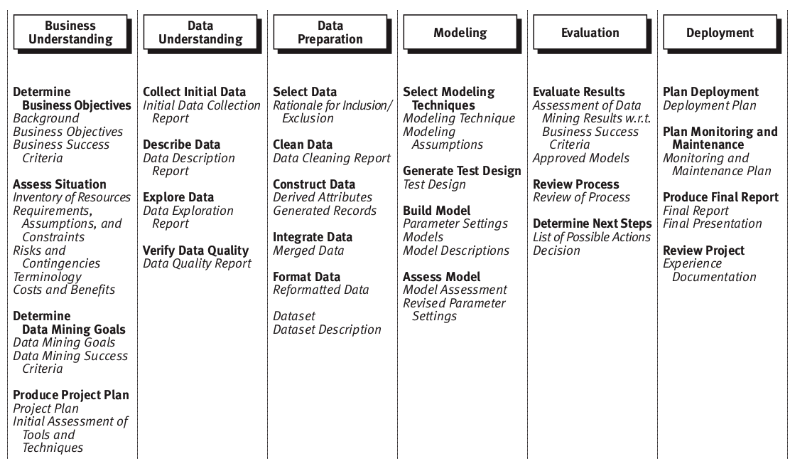
\includegraphics[scale=0.33]{images/crisp-dm-fig.png}
\end{frame}
%----------------------------------------------------------------------------------------
\begin{frame}{Goals of Data Exploration}
\begin{itemize}
	\setlength\itemsep{0.25cm}
	\item Understand the \textbf{structure} of the dataset:
		\begin{itemize}
			\item Number of features (columns) and instances / observations(rows).
			\item Types of variables: categorical vs. continuous.
			\item Summary statistics: mean, median, standard deviation, missing values, etc..
		\end{itemize}
	\item \textbf{Detect potential issues}:
		\begin{itemize}
			\item Missing or inconsistent values.
			\item Outliers or extreme values.
			\item Data entry errors, duplicate records.
		\end{itemize}
	\item Guide data \textbf{preprocessing decisions}:
		\begin{itemize}
			\item Whether normalization or standardization is needed.
			\item Features selection \& alignment with objective.
		\end{itemize}
\end{itemize}
\end{frame}
%----------------------------------------------------------------------------------------
\section{Data Quality Report}
\begin{frame}{The Data Quality Report}
\begin{itemize}
    \setlength\itemsep{0.5cm}
    \item A structured summary of dataset characteristics.
    \item Helps identify \textbf{inconsistencies, missing data, and errors} before modeling.
    \item Serves as a \textbf{documentation tool} for tracking dataset changes.
    \item Provides insights into whether additional \textbf{data cleaning or preprocessing} is needed.
\end{itemize}
\end{frame}
%----------------------------------------------------------------------------------------

\begin{frame}{Components of a Data Quality Report}
\begin{itemize}
    \setlength\itemsep{0.5cm}
    \item \textbf{Tabular Summaries for Features}
    \begin{itemize}
    \setlength\itemsep{0.25cm}
        \item Overview of numerical and categorical variables.
        \item Summary statistics:
        \begin{itemize}
        \setlength\itemsep{0.25cm}
            \item \textbf{Continuous variables}: mean, median, standard deviation, min, max, quartiles.
            \item \textbf{Categorical variables}: unique values, mode, frequency distribution.
        \end{itemize}
    \end{itemize}
\end{itemize}
\end{frame}
%----------------------------------------------------------------------------------------

\begin{frame}{Statistical Measures for Data Quality}
\begin{itemize}
    \setlength\itemsep{0.5cm}
    \item \textbf{Missing values}: Count and percentage of missing data.
    \item \textbf{Cardinality}: Number of unique values in categorical features.
    \item \textbf{Outliers}: Extreme values outside expected ranges.
    \item \textbf{Correlations}: Detecting redundant features.
\end{itemize}
\end{frame}
%----------------------------------------------------------------------------------------

\begin{frame}{Data Visualizations for Exploration}
\begin{itemize}
    \setlength\itemsep{0.5cm}
    \item \textbf{Histograms}: Visualize feature distributions.
    \item \textbf{Box Plots}: Identify outliers and spread of data.
    \item \textbf{Bar Charts}: Categorical feature distributions.
    \item \textbf{Scatter Plots}: Detect relationships between numerical variables.
\end{itemize}
\end{frame}
%----------------------------------------------------------------------------------------

\begin{frame}{Case Study: Motor Insurance Fraud Detection}
\begin{itemize}
    \setlength\itemsep{0.5cm}
    \item \textbf{Example scenario}: Predict fraudulent motor insurance claims.
    \item \textbf{Initial data review}:
    \begin{itemize}
        \item Identify missing or inconsistent claim details.
        \item Assess frequency distributions of claim types.
        \item Detect patterns in high-claim amounts and fraudulent cases.
    \end{itemize}
    \item \textbf{Goal}: Guide data preprocessing for better fraud detection models.
\end{itemize}
\end{frame}
%----------------------------------------------------------------------------------------
\begin{frame}{Case Study: Motor Insurance Fraud Detection}
\centering
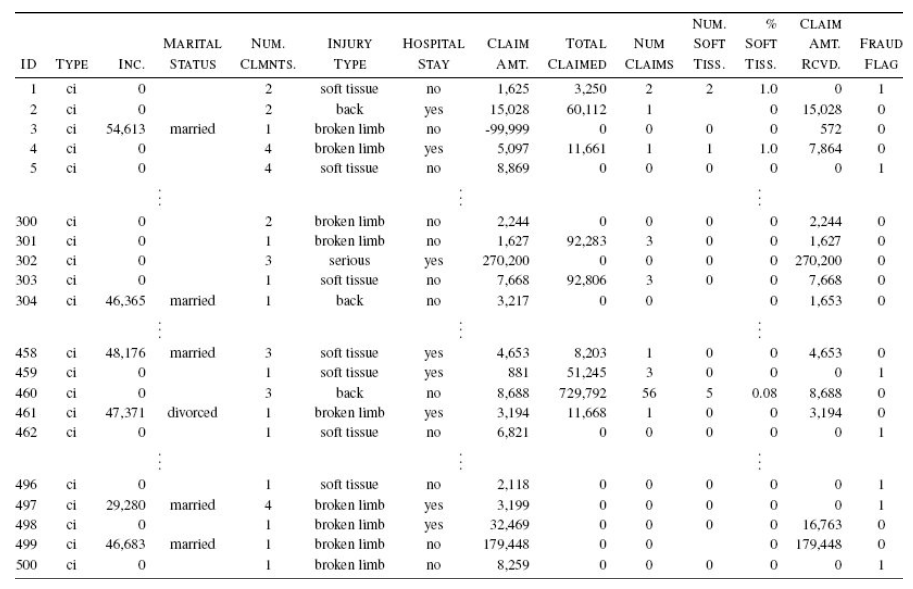
\includegraphics[scale=0.32]{images/motor_dat.png}
\captionof{figure}{Portion of Motor Insurance Claim Data}
\end{frame}
%----------------------------------------------------------------------------------------
\begin{frame}{Case Study: Motor Insurance Fraud Detection}
\centering
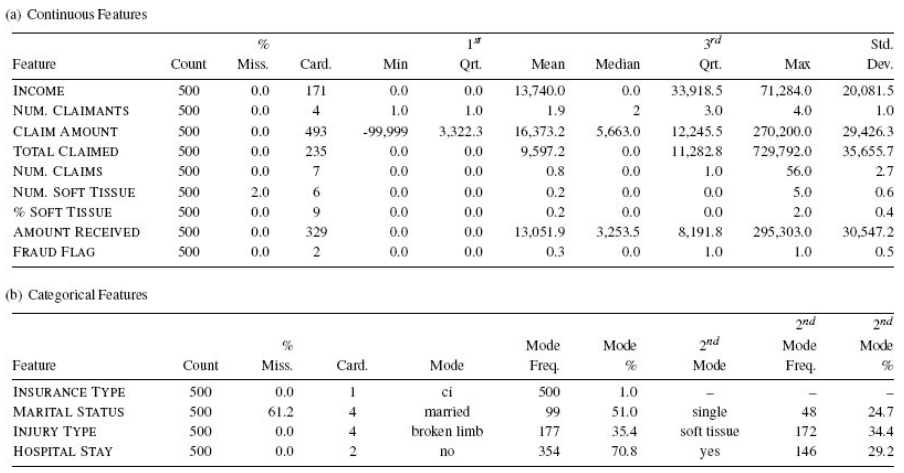
\includegraphics[scale=0.32]{images/motor_rep.png}
\captionof{figure}{Data Quality Report for Motor Insurance Claim Data}
\end{frame}
%----------------------------------------------------------------------------------------
\begin{frame}{Case Study: Motor Insurance Fraud Detection}
\centering
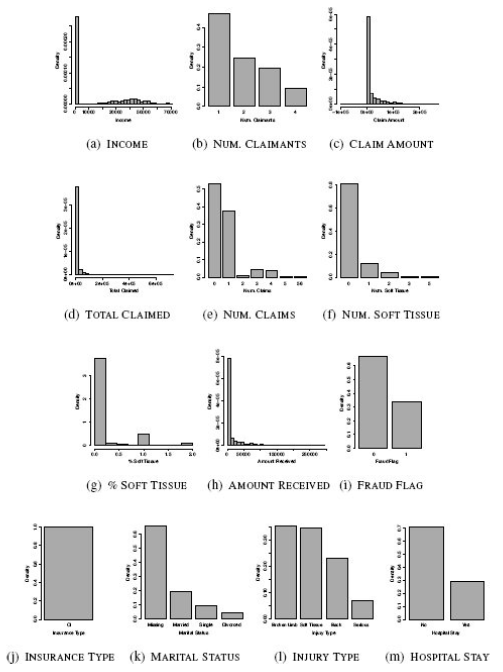
\includegraphics[scale=0.32]{images/motor_fig.png}
\captionof{figure}{Data Quality Figures for Motor Insurance Claim Data}
\end{frame}
%----------------------------------------------------------------------------------------
\section{Getting to Know the Data}
\begin{frame}{Understanding and Exploring the Data}
\begin{itemize}
    \setlength\itemsep{0.5cm}
    \item Identify the types and distributions of features in the dataset.
    \item Differentiate between \textbf{continuous} and \textbf{categorical} features.
    \item Assess skewness, central tendency, and variability.
    \item Use statistical summaries and visual tools (histograms, bar charts, box plots) to examine data characteristics.
\end{itemize}
\end{frame}
%----------------------------------------------------------------------------------------

\begin{frame}{Feature Types and Statistical Measures}
\begin{itemize}
    \setlength\itemsep{0.5cm}
    \item \textbf{Continuous Features}:
    \begin{itemize}
        \item Examples: Age, Income, Temperature.
        \item Use histograms, box plots, and summary statistics (mean, median, standard deviation) for insights.
    \end{itemize}
    \item \textbf{Categorical Features}:
    \begin{itemize}
        \item Examples: Gender, Product Category.
        \item Use frequency tables, bar plots, and pie charts to explore distributions.
        \item Detect class imbalances that may impact predictive modeling.
    \end{itemize}
\end{itemize}
\end{frame}
%----------------------------------------------------------------------------------------

\subsection{The Normal Distribution}
\begin{frame}{The Normal Distribution: Overview}
\begin{itemize}
    \setlength\itemsep{0.5cm}
    \item Defined by two parameters:
    \begin{itemize}
        \item \textbf{Mean ($\mu$)}: The central location of the distribution.
        \item \textbf{Standard deviation ($\sigma$)}: Measures the spread of data.
    \end{itemize}
    \item Characterized by its symmetric, bell-shaped curve, and common in natural phenomena such as heights, test scores, and financial returns.
\end{itemize}
\centering
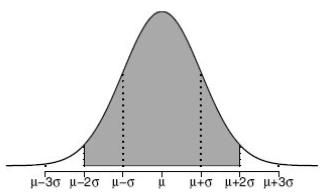
\includegraphics[scale=0.4]{images/normal_dist.png}
\end{frame}
%----------------------------------------------------------------------------------------

\begin{frame}{The Normal Distribution: Properties}
\begin{itemize}
    \setlength\itemsep{0.25cm}
    \item \textbf{Empirical Rule}:
    \begin{itemize}
        \item 68\% of data falls within $1\sigma$ of the mean.
        \item 95\% within $2\sigma$.
        \item 99.7\% within $3\sigma$.
    \end{itemize}
    \item \textbf{Statistical Applications}:
    \begin{itemize}
        \item Basis for parametric statistical tests (e.g., t-tests, ANOVA).
        \item Used in probabilistic modeling and hypothesis testing.
    \end{itemize}
    \item \textbf{Central Limit Theorem (CLT)}:
    \begin{itemize}
        \item Explains why sample means tend to be normally distributed.
        \item Justifies using normal-based methods in inferential statistics ($n\geq30$).
    \end{itemize}
\end{itemize}
\end{frame}
%----------------------------------------------------------------------------------------

\begin{frame}{Detecting and Handling Deviations from Normality}
\begin{itemize}
    \setlength\itemsep{0.25cm}
    \item \textbf{Identifying Non-Normality}:
    \begin{itemize}
        \item Visual methods: Histograms, QQ-plots.
        \item Statistical tests: Shapiro-Wilk, Kolmogorov-Smirnov.
    \end{itemize}
    \item \textbf{Implications of Non-Normal Data}:
    \begin{itemize}
        \item May violate assumptions of statistical models.
        \item Can impact performance of machine learning algorithms.
    \end{itemize}
    \item \textbf{Transformations to Normalize Data}:
    \begin{itemize}
        \item Log transformation for right-skewed data.
        \item Box-Cox transformation for general adjustments.
        \item Standardization (z-score normalization) for mean-centering.
    \end{itemize}
\end{itemize}
\end{frame}
%----------------------------------------------------------------------------------------

\begin{frame}{Different Distributions}
\centering
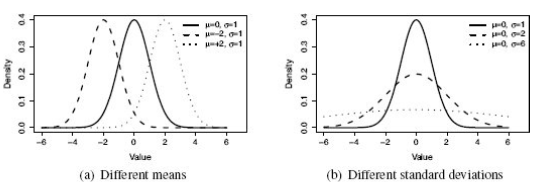
\includegraphics[scale=0.33]{images/diff_sds}
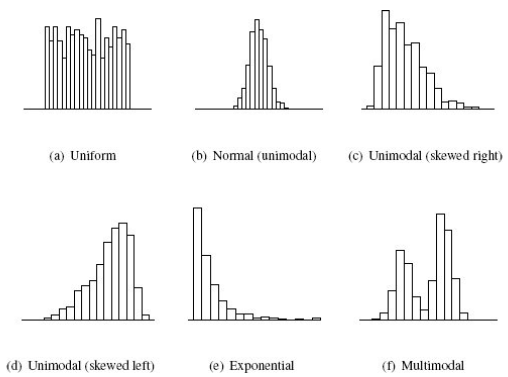
\includegraphics[scale=0.43]{images/diff_distributions}
\end{frame}
%----------------------------------------------------------------------------------------
\section{Identifying Data Quality Issues}
\begin{frame}{Identifying Data Quality Issues}
\begin{itemize}
    \setlength\itemsep{0.25cm}
    \item Poor data quality can negatively impact model performance and insights.
    \item Key data quality issues include:
    \begin{itemize}
        \item Missing values
        \item Irregular cardinality
        \item Outliers and anomalies
    \end{itemize}
    \item Addressing these issues is crucial for reliable data-driven decision making.
\end{itemize}
\vspace{0.1cm}
\centering
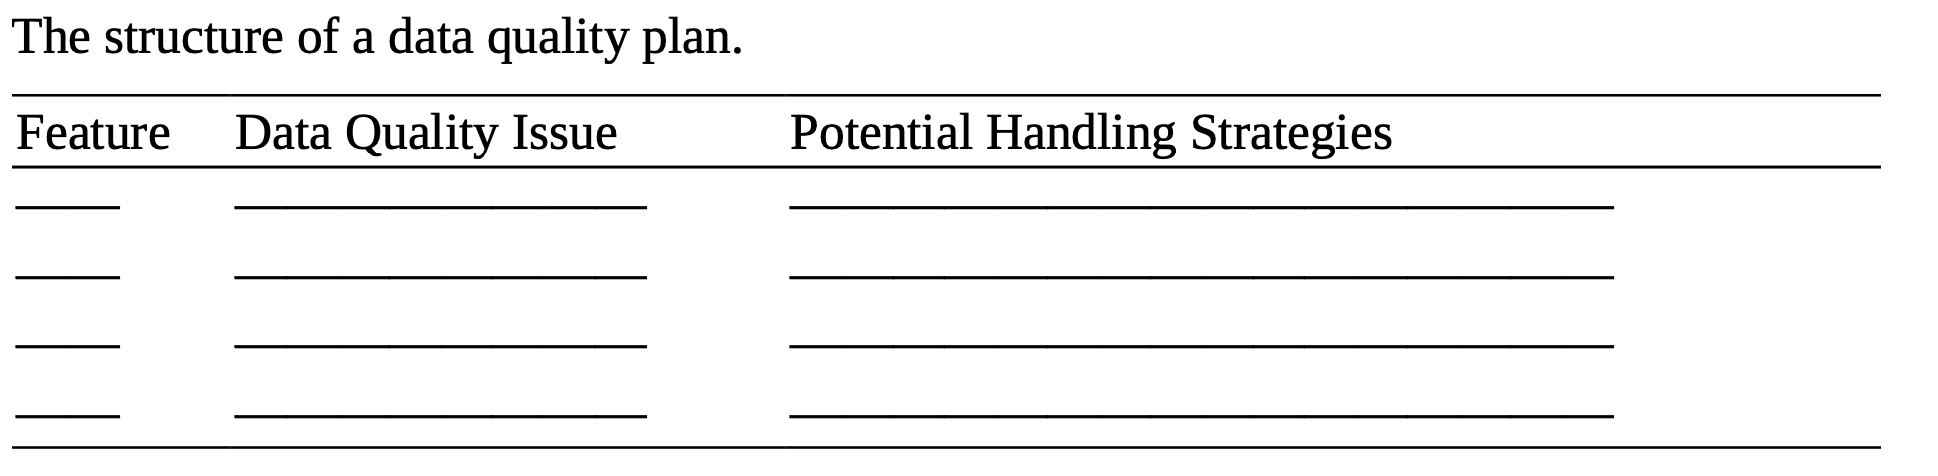
\includegraphics[scale=0.33]{images/data_quality_plan.png}
\end{frame}
%----------------------------------------------------------------------------------------

\begin{frame}{Missing Values: Causes and Consequences}
\begin{itemize}
    \setlength\itemsep{0.25cm}
    \item \textbf{Causes of Missing Data}:
    \begin{itemize}
        \item Human error in data entry.
        \item Data corruption or loss during processing.
        \item Non-response in surveys or experiments.
    \end{itemize}
    \item \textbf{Types of Missing Data}:
    \begin{itemize}
        \item Missing Completely at Random (MCAR)
        \item Missing at Random (MAR)
        \item Missing Not at Random (MNAR)
    \end{itemize}
    \item \textbf{Consequences}:
    \begin{itemize}
        \item Reduces data usability.
        \item Can bias analytical results if not handled properly.
    \end{itemize}
\end{itemize}
\end{frame}
%----------------------------------------------------------------------------------------

\begin{frame}{Irregular Cardinality in Categorical Variables}
\begin{itemize}
    \setlength\itemsep{0.25cm}
    \item \textbf{Definition}: Cardinality refers to the number of unique values a categorical feature can take.
    \item \textbf{Potential Issues}:
    \begin{itemize}
        \item High cardinality: Many unique values can cause overfitting and increase model complexity.
        \item Low cardinality: May indicate redundancy or poor feature utility.
    \end{itemize}
    \item \textbf{Detection Methods}:
    \begin{itemize}
        \item Frequency distribution analysis.
        \item Visualizing unique values with bar plots.
    \end{itemize}

\end{itemize}
\end{frame}
%----------------------------------------------------------------------------------------

\begin{frame}{Outliers and Anomalies}
\begin{itemize}
    \setlength\itemsep{0.25cm}
    \item \textbf{Definition}: Outliers are extreme values that deviate significantly from the rest of the data.
    \item \textbf{Causes}:
    \begin{itemize}
        \item Data entry errors.
        \item Genuine rare events.
        \item Sensor or measurement errors.
    \end{itemize}
    \item \textbf{Detection Methods}:
    \begin{itemize}
        \item Statistical techniques: Z-scores, IQR method.
        \item Visualization techniques: Box plots, scatter plots.
    \end{itemize}
\end{itemize}
\end{frame}

%----------------------------------------------------------------------------------------
\section{Handling Data Quality Issues}

\begin{frame}{Handling Data Quality Issues}
\begin{itemize}
    \setlength\itemsep{0.5cm}
    \item Addressing data quality issues improves model reliability and accuracy.
    \item Common techniques include:
    \begin{itemize}
        \item Imputing missing values.
        \item Managing irregular cardinality in categorical features.
        \item Handling outliers effectively.
    \end{itemize}
	\item How could prediction be used to fill missing fields for imputation? Could correlation help with this?
\end{itemize}
\end{frame}
%----------------------------------------------------------------------------------------

\begin{frame}{Handling Missing Values}
\begin{itemize}
    \setlength\itemsep{0.5cm}
    \item \textbf{Strategies for Handling Missing Data}:
    \begin{itemize}
        \item \textbf{Deletion}: Remove rows or columns with excessive missing values.
        \item \textbf{Imputation}:
        \begin{itemize}
            \item Mean, median, or mode substitution.
            \item Predictive modeling (e.g., KNN imputation, regression imputation).
        \end{itemize}
        \item \textbf{Indicator Variable Method}: Add a new feature indicating missingness.
    \end{itemize}
    \item Consider the missing data mechanism (MCAR, MAR, MNAR) before applying a strategy.
\end{itemize}
\end{frame}
%----------------------------------------------------------------------------------------

\begin{frame}{Managing Irregular Cardinality}
\begin{itemize}
    \setlength\itemsep{0.25cm}
    \item \textbf{High Cardinality Issues}:
    \begin{itemize}
        \item Increases computational complexity and risk of overfitting.
        \item Common in features like zip codes, product IDs, or names.
    \end{itemize}
    \item \textbf{Techniques for Handling High Cardinality}:
    \begin{itemize}
        \item \textbf{Grouping}: Merge rare categories into an "Other" category.
        \item \textbf{Encoding}:
        \begin{itemize}
            \item One-hot encoding (useful for small cardinality features).
            \item Target encoding or frequency encoding for high cardinality features.
        \end{itemize}
    \end{itemize}
\end{itemize}
\end{frame}
%----------------------------------------------------------------------------------------

\begin{frame}{Handling Outliers and Anomalies}
\begin{itemize}
    \setlength\itemsep{0.25cm}
    \item \textbf{Identifying Outliers}:
    \begin{itemize}
        \item Statistical methods: Z-score, IQR method.
        \item Visual methods: Box plots, scatter plots.
    \end{itemize}
    \item \textbf{Strategies for Handling Outliers}:
    \begin{itemize}
        \item \textbf{Truncation}: Cap values within a predefined range.
        \item \textbf{Transformation}: Apply log transformation to reduce skewness.
        \item \textbf{Model-based approaches}: Use robust algorithms less sensitive to outliers (e.g., decision trees, random forests).
    \end{itemize}
    \item Choose the appropriate method based on whether the outliers are data errors or meaningful anomalies.
\end{itemize}
\end{frame}
%----------------------------------------------------------------------------------------

\section{Advanced Data Exploration}

\begin{frame}{Advanced Data Exploration}
\begin{itemize}
    \setlength\itemsep{0.5cm}
    \item Data exploration goes beyond basic summaries to uncover deeper patterns that impact model performance.
    \item Traditional summary statistics provide useful insights, but advanced techniques help:
    \begin{itemize}
        \item Detect complex relationships between variables.
        \item Identify hidden structures in the dataset.
        \item Improve feature selection and engineering decisions.
    \end{itemize}
    \item Why it matters:
    \begin{itemize}
        \item Machine learning models rely on clean, well-structured input features.
        \item Poorly understood data can lead to bias, overfitting, and misleading conclusions.
    \end{itemize}
\end{itemize}
\end{frame}
%----------------------------------------------------------------------------------------


\begin{frame}{Visualizing Relationships Between Features}
\begin{itemize}
    \setlength\itemsep{0.25cm}
    \item Graphical representations reveal hidden patterns and dependencies.
    \item Common visualization techniques:
    \begin{itemize}
        \item \textbf{Scatter Plots}: Show relationships between continuous variables.
        \item \textbf{Pair Plots}: Matrix of scatter plots for multiple features.
        \item \textbf{Box Plots}: Compare distributions across categorical groups.
        \item \textbf{Heatmaps}: Visualize correlation matrices.
    \end{itemize}
\end{itemize}
\centering
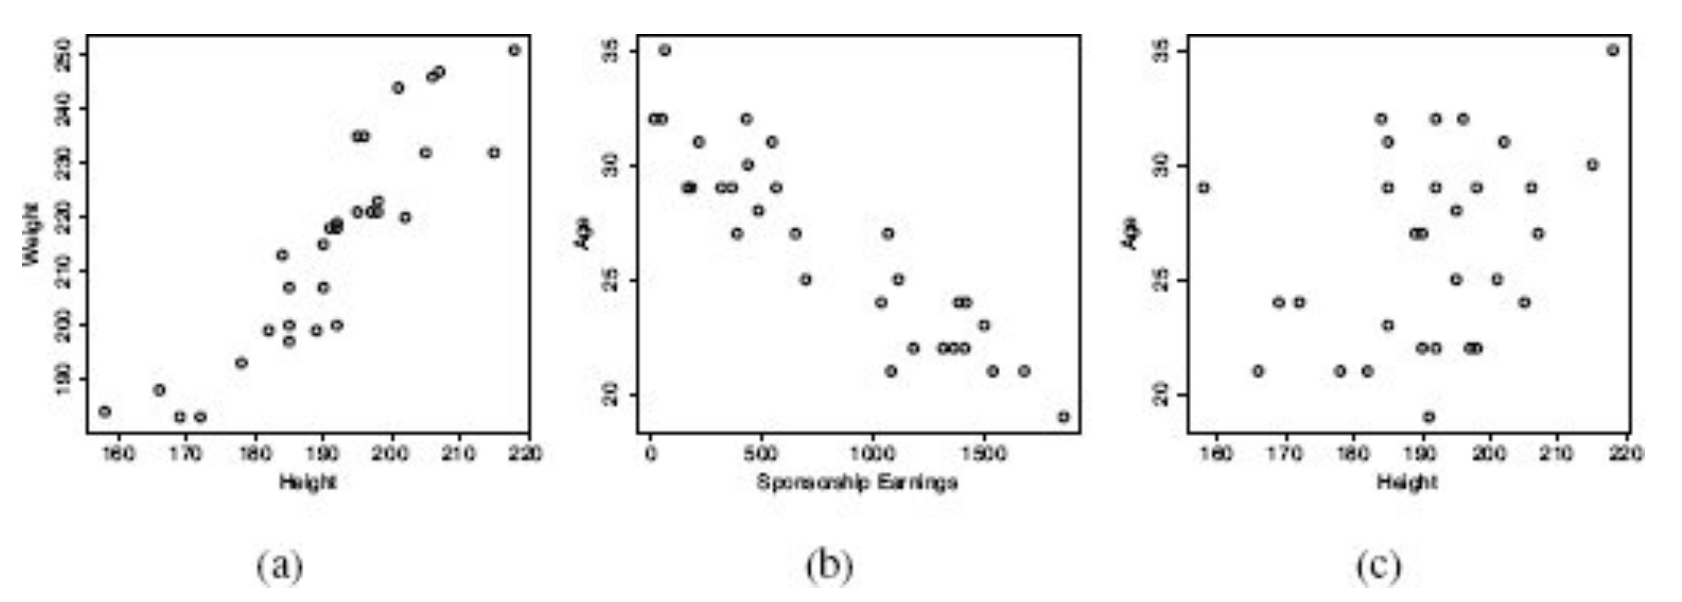
\includegraphics[scale=0.33]{images/covariates.png}
\end{frame}
%----------------------------------------------------------------------------------------
\begin{frame}
\centering
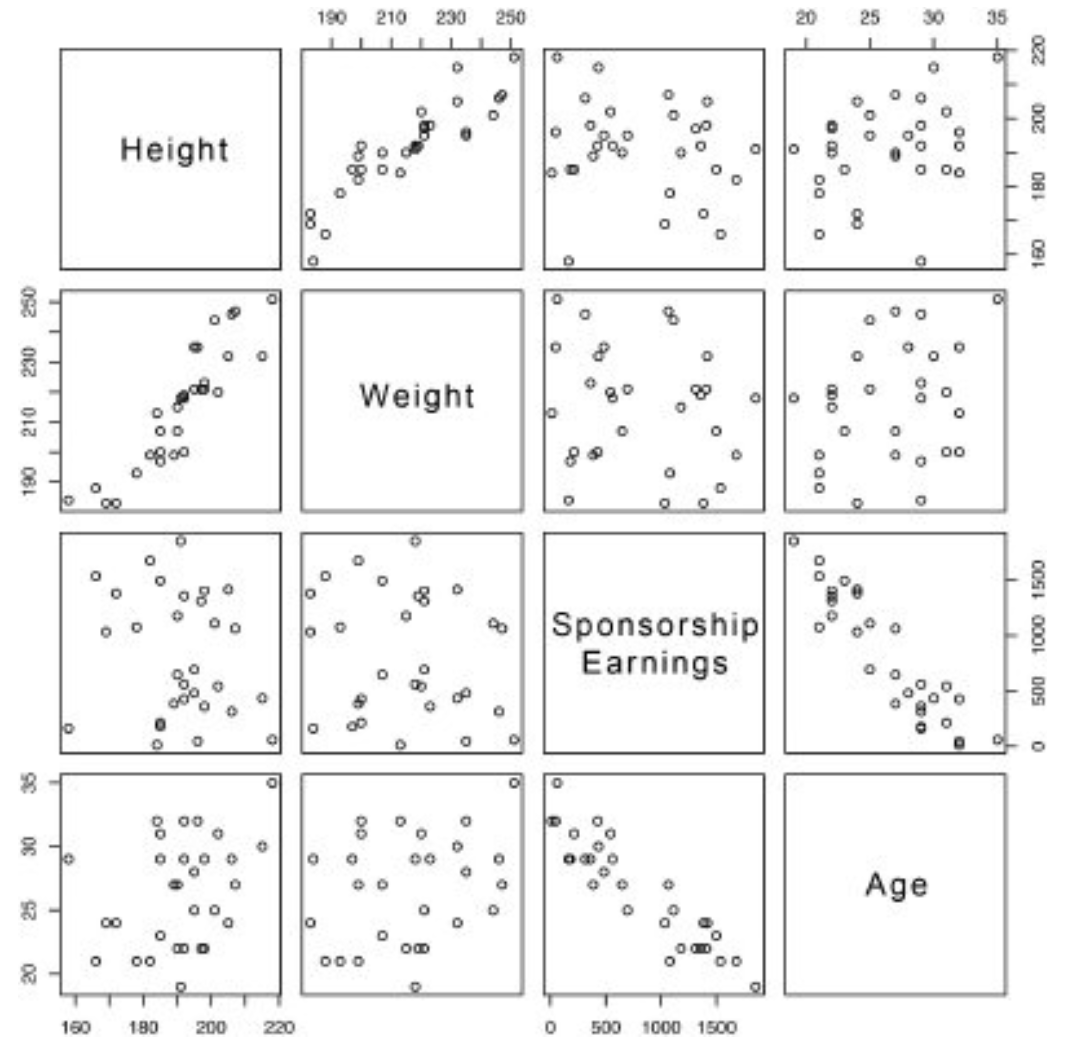
\includegraphics[scale=0.45]{images/splot_mat.png}
\end{frame}
%----------------------------------------------------------------------------------------
\begin{frame}
\centering
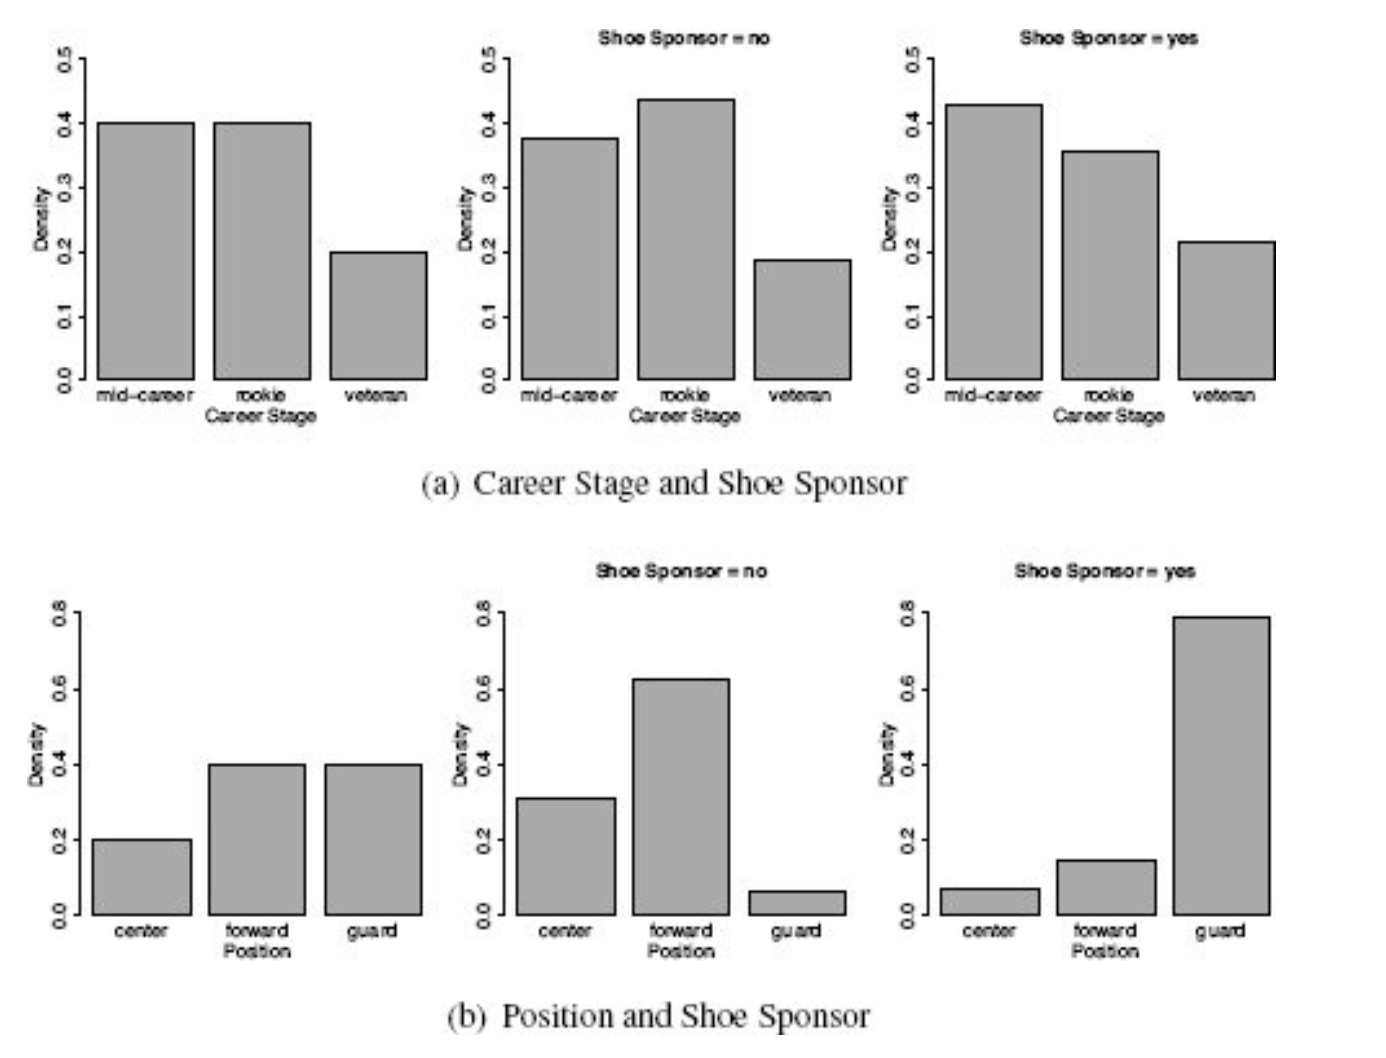
\includegraphics[scale=0.45]{images/hist_grid.png}
\end{frame}
%----------------------------------------------------------------------------------------

\begin{frame}{Measuring Covariance and Correlation}
\begin{itemize}
    \setlength\itemsep{0.25cm}
    \item \textbf{Covariance}:
    \begin{itemize}
        \item Measures the direction of a linear relationship between two variables.
        \item A positive covariance indicates both variables increase together.
        \item A negative covariance indicates one increases while the other decreases.
    \end{itemize}
    \item \textbf{Correlation}:
    \begin{itemize}
        \item Standardized measure of the strength and direction of a relationship.
        \item Ranges from -1 (strong negative) to +1 (strong positive).
        \item Pearson, Spearman, and Kendall correlation methods.
    \end{itemize}
\end{itemize}
\end{frame}
%----------------------------------------------------------------------------------------
\begin{frame}
\centering
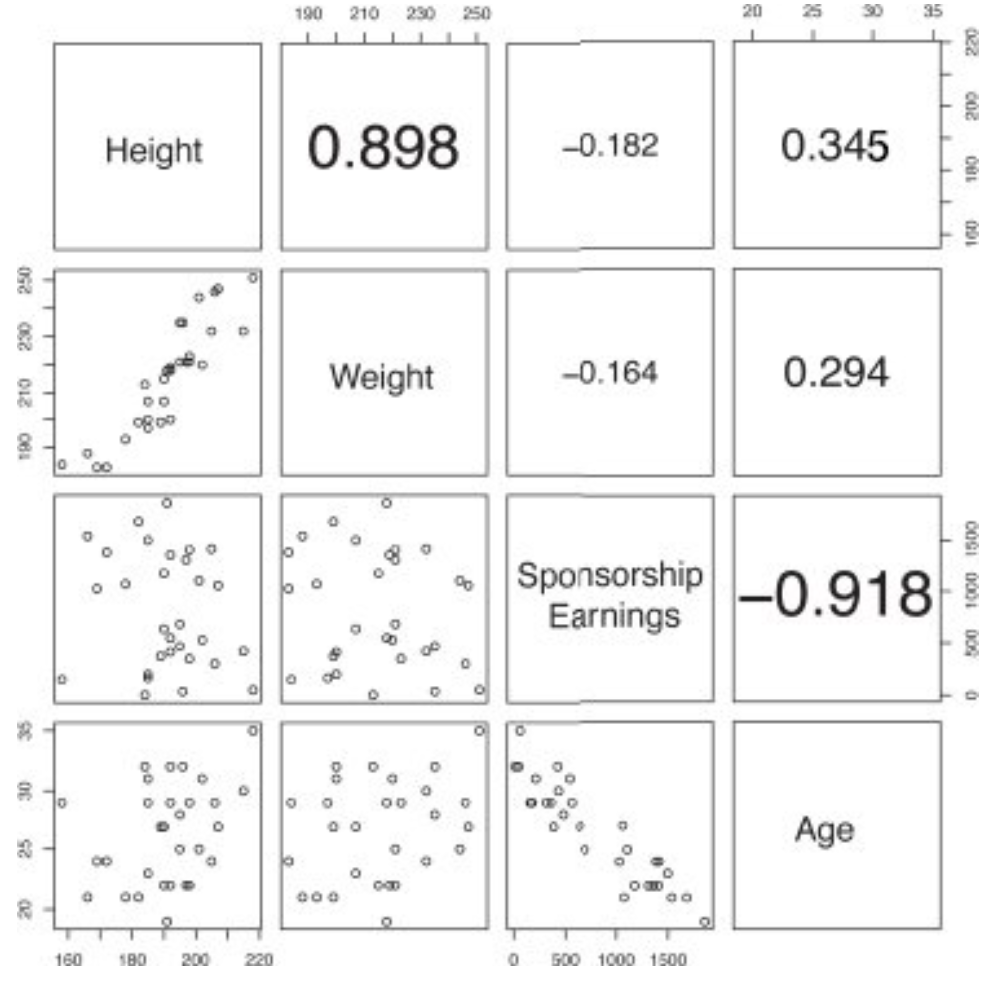
\includegraphics[scale=0.4]{images/cov_mat.png}
\captionof{figure}{A scatter plot matrix showing scatter plots of the continuous features from the professional
basketball team dataset with correlation coefficients included.}
\end{frame}
%----------------------------------------------------------------------------------------

\begin{frame}{Identifying Multicollinearity}
\begin{itemize}
    \setlength\itemsep{0.25cm}
    \item Multicollinearity occurs when independent variables are highly correlated.
    \item Issues caused by multicollinearity:
    \begin{itemize}
        \item Inflates variance in regression coefficients.
        \item Reduces model interpretability.
    \end{itemize}
    \item Detection Methods:
    \begin{itemize}
        \item Variance Inflation Factor (VIF): Higher VIF values indicate multicollinearity.
        \item Eigenvalue decomposition of correlation matrix.
    \end{itemize}
    \item Handling multicollinearity:
    \begin{itemize}
        \item Removing highly correlated features.
        \item Principal Component Analysis (PCA) for dimensionality reduction.
    \end{itemize}
\end{itemize}
\end{frame}
%----------------------------------------------------------------------------------------
\section{Lab}
\subsection{GitHub Introduction}

\begin{frame}{Lab: Introduction to Git and GitHub}
\begin{itemize}
    \setlength\itemsep{0.5cm}
    \item \textbf{Git}: A command-line version control system for tracking changes in files. "Saves Progress" in projects, and allows for version roll-backs. 
    \item \textbf{GitHub}: A cloud-based platform for hosting Git repositories. Stores code for personal or public sharing. The standard for sharing projects and code.
    \item Benefits of Git/GitHub:
    \begin{itemize}
        \item Enables collaboration on projects by managing user privleges by project.
        \item Provides a detailed history of changes.
        \item Facilitates code backup and versioning.
    \end{itemize}
\end{itemize}
\end{frame}
%----------------------------------------------------------------------------------------

\begin{frame}{Setting Up a Local Repository with GitHub}
\centering
\href{run:./Getting Started with Git on Windows and MacOS.pdf}{\color{blue} \underline{Let's Set-Up Git/Github for our Projects.}}
\vspace{0.2cm}

\includegraphics[scale=0.2]{images/github_git.jpg}
\end{frame}


\begin{frame}{Basic Git Command-Line Workflow}
\begin{itemize}
    \setlength\itemsep{0.25cm}
    \item A simple workflow for tracking changes using Git:
    \begin{enumerate}
        \item \textbf{Initialize a repository}: `git init`
        \item \textbf{Check the status}: `git status`
        \item \textbf{Stage changes}: `git add $<$file$>$`
        \item \textbf{Commit changes}: `git commit -m "Commit message"`
        \item \textbf{View commit history}: `git log`
        \item \textbf{Push to remote repository}: `git push`
    \end{enumerate}
\end{itemize}
\vspace{0.25cm}
\centering
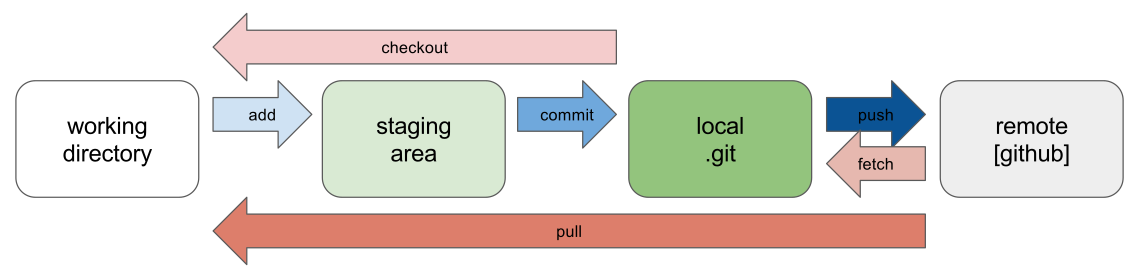
\includegraphics[scale=0.33]{images/git_workflow.png}
\end{frame}


\subsection{Data Exploration \& Tidyverse}

\begin{frame}{Lab: Data Exploration \& Tidyverse}
\begin{itemize}
	\setlength\itemsep{0.5cm}
	\item Worksheet

\end{itemize}
\end{frame}
%----------------------------------------------------------------------------------------


\end{document}